\Figure{coverage_moll} {The coverage of the BGPS.  The background
greyscale is IRAS 100 \mum.  
%[James, team: is there a better figure 
%option?]
%[I think this is fine. For print, you can try a black line instead
%of red. NJE]
}{fig:Coverage}{1.0}

% Figure 3
\Figure{bolocam_bandpass}{The Bolocam 1.1 mm bandpass (thick line).  Bright
molecular emission lines are shown at their rest frequencies.  For
comparison, the MAMBO-2 bandpass is shown as a thin line.  Note that
the Bolocam passband rejects $>90\%$ of the $^{12}$CO flux, leaving
our continuum measurements largely uncontaminated.  SO$_2$ and
CH$_3$OH lines are likely strong contributors to line flux in the
passband.  \citet{nummelin1998} found that 22\% of the flux density in
one pointing towards Sgr B2 was from lines, and \citet{yoshida2005}
reported $>40\%$ in Orion A from line emission over the 260-328 GHz
band. Other lines lying in the Bolocam passband include CS($5\to4$)
and ($6\to5$) (245 and 293 GHz), HCN($3\to2$) (265 GHz) and
HCO$^+(3\to2)$ (267 GHz).  }
% A follow-up project will attempt to determine the contribution of lines
% to the BGPS flux density measurements.}
{fig:Bandpass}{1.0}

% Figure 4
\FigureTwo{bolosens050904_o32}{scan_10deg}{Left: the position,
ellipticity and relative response of the detectors in the Bolocam
focal plane as mapped to the sky.  Right: The effect of field rotation
on the coverage obtained via Bolocam raster scans.  The array is held
fixed during a scan, but is rotated relative to the scan direction
such that the sampling is most uniform by attaining the best sampling
in the cross-scan direction.}{fig:Array}{1.0}

\FigureTwo{fluxcal_errorbars}{calib_vs_dc}
%{rel_flux_cal_050303_ob3_to_050405_o66}
%{calibration_plot_2004}
{Left: Average calibration curve [V/Jy] versus the mean detector
voltage, a proxy for atmospheric loading.  Red points are observations
of Mars and black of Uranus.  The black line is a 2nd-order fit with
0,0 forced (no response if no measurable potential difference) .
Right: Scaling of the relative response to the atmosphere for a single
detector compared to the array median.  Outliers are from noisy scans
that are strongly downweighted.}{fig:CalibrationCurves}{1.0}

% 6
\Figure{relsens_cal}{An illustration of the relative sensitivity
calibration using the atmosphere as a calibrator.  Black is the median
over all bolometers (the 1st-order atmosphere model), red and green are
individual bolometers. a. before and b. after applying the relative
calibration.  Note the improved agreement.}{fig:Flatfield}{1.0}

% 7
\Figure{cygnus_flux_comparison}{A comparison of the fluxes extracted
in the same aperture from the \citet{motte07} MAMBO map and the
Bolocam map of this paper. }{fig:CygnusComparison}{1.0}


% 8
% -----------------------------------------------------------------------------
\FigureTwo{plane_astrometry}{pointing_model_skydist}{Left: The
distribution of absolute reference sources (crosses) in the Galactic
Plane (Appendix \ref{app:PointingCalibrators}).  Also shown (crosses)
are the locations of bright, isolated, compact sources for comparison
with other surveys, as given in Appendix \ref{app:ReferenceSources}.
Right: The distribution of the pointing calibration sources across the
local sky in Hawaii during July 2007 (epoch V) when the pointing model
was constructed.  }{fig:PointingCalibrators}{1.0}
% -----------------------------------------------------------------------------

% 9
% -----------------------------------------------------------------------------
\begin{figure}
  \subfigure[The pointing model correction (left) and residuals (right) for
  Epoch V, from which the master reference images were derived for subsequent
  alignment.  The red line indicates the fitted model. 510 pointing sources
  were included, and the final RMS was 5.77\arcsec in altitude and 3.21\arcsec
  in azimuth, or a total RMS offset of 6.6\arcsec.  No systematic offset with
  altitude was found.]
{\label{fig:PointingModel-a}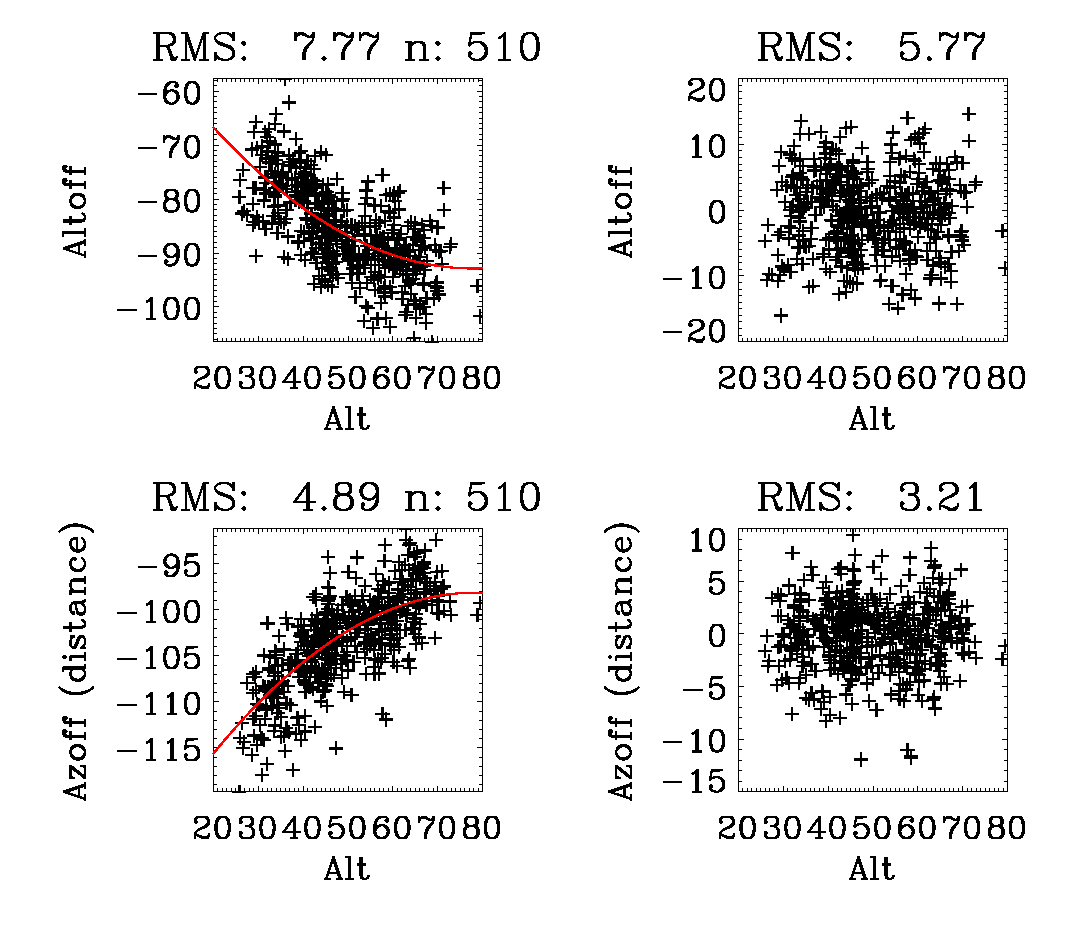
\includegraphics[scale=0.9]{paper_models_0707}}\\

  \subfigure[The residuals of the pointing model.  The Gaussian fits have
  $\sigma = 5.94,2.92$ in altitude offset and azimuth offset respectively.]
{\label{fig:PointingModel-b}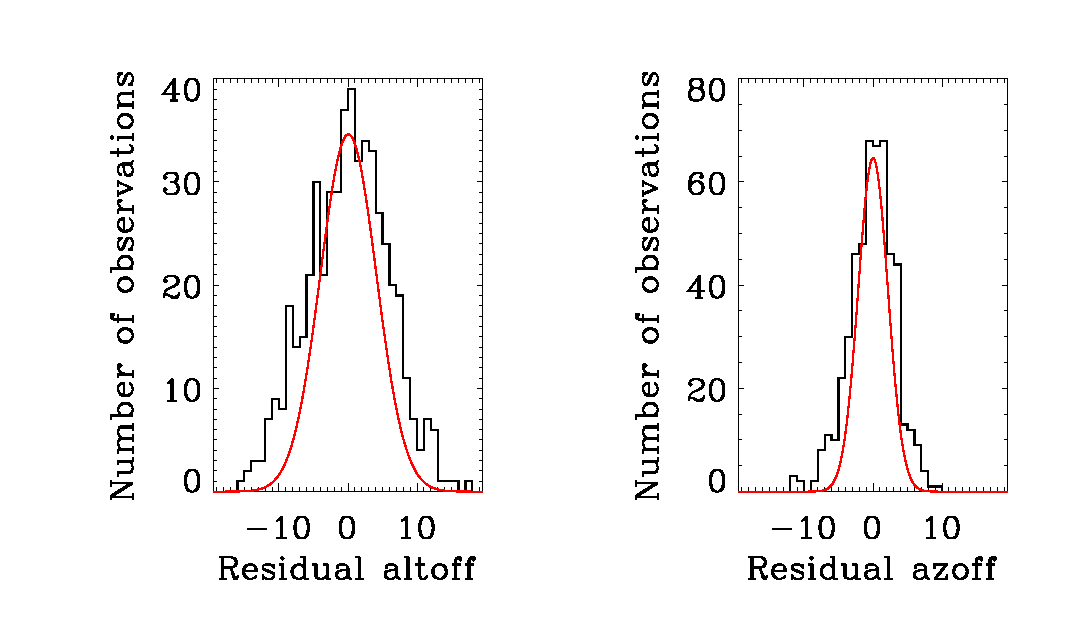
\includegraphics[scale=0.9]{paper_gaussian_0707}}

\caption{The Bolocam pointing model for Epoch V.}
\label{fig:PointingModel}
\end{figure}
% -----------------------------------------------------------------------------


% 10
% -----------------------------------------------------------------------------
\begin{figure}

  \subfigure[{\it Left}: the Bolocam map in a portion of the $\lon=30$
  field.  {\it Right}: the SLC maps in the same region.  The green
  contours on the Bolocam map indicate the positions of the SLC
  sources.  Negative bowls in the image are forced to zero before
  cross-correlating.  ]
  {\label{fig:SCUBAPointingComparison-a}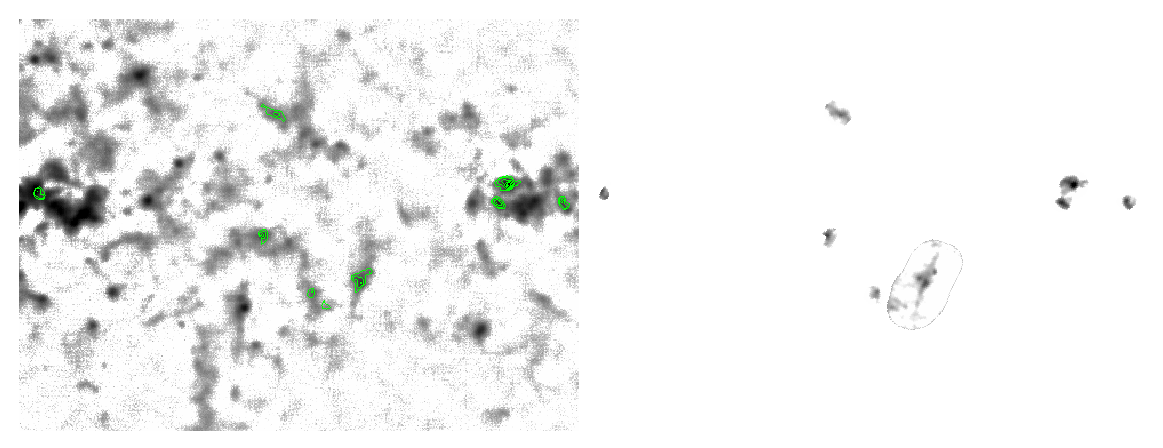
\includegraphics[scale=0.8]
  {scuba_bolocam_l030}}

  \begin{tabular}{cc}

  \subfigure[The cross-correlation map of the BGPS and SLC maps in
  Figure \ref{fig:SCUBAPointingComparison-a}. {\bf to be replaced with
  correct map}]
  {\label{fig:SCUBAPointingComparison-b}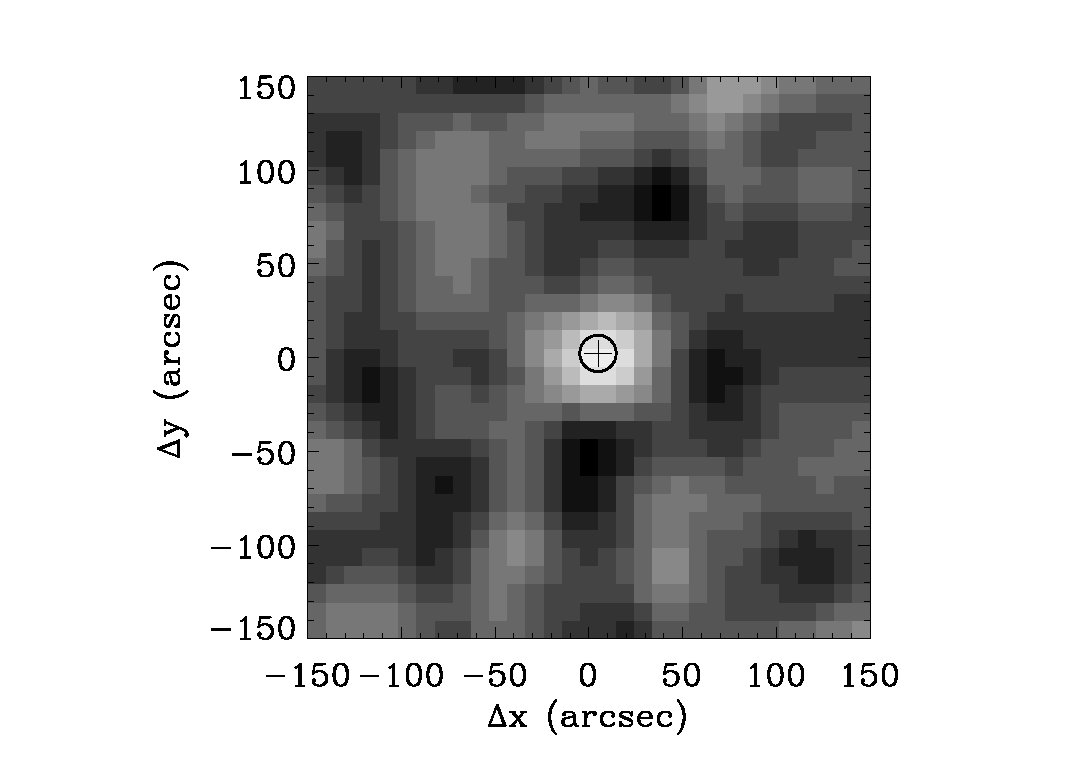
\includegraphics[scale=0.45]
  {xcorr_standin}}

  \subfigure[The measured offset between Bolocam and SCUBA Legacy
sources \citep{difrancesco08}, using the method described in Setion
\ref{sec:SCUBAPointingComparison}.  The circle indicates the $1\sigma$
region, which is also consistent with the error derived from the
internal Bolocam pointing model.]
{\label{fig:SCUBAPointingComparison-c}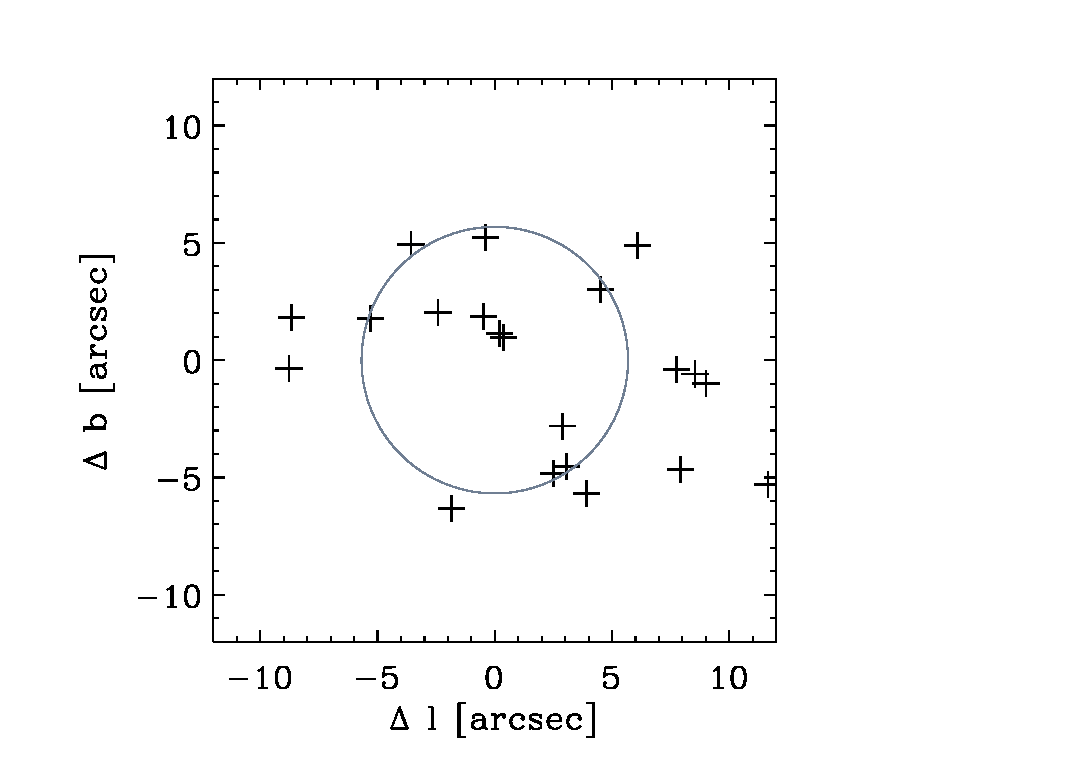
\includegraphics[scale=0.45]
{scuba_pointing_offsets}}

\end{tabular}

\caption{Comparing the Bolocam positions to those of the SCUBA Legacy Catalog.}
\label{fig:SCUBAPointingComparison}
\end{figure}
% -----------------------------------------------------------------------------

\setcounter{subfig}{1}
\renewcommand{\thefigure}{\arabic{figure}\alph{subfig}}

\begin{figure}
  \begin{minipage}{6.5in}
    \begin{center}
      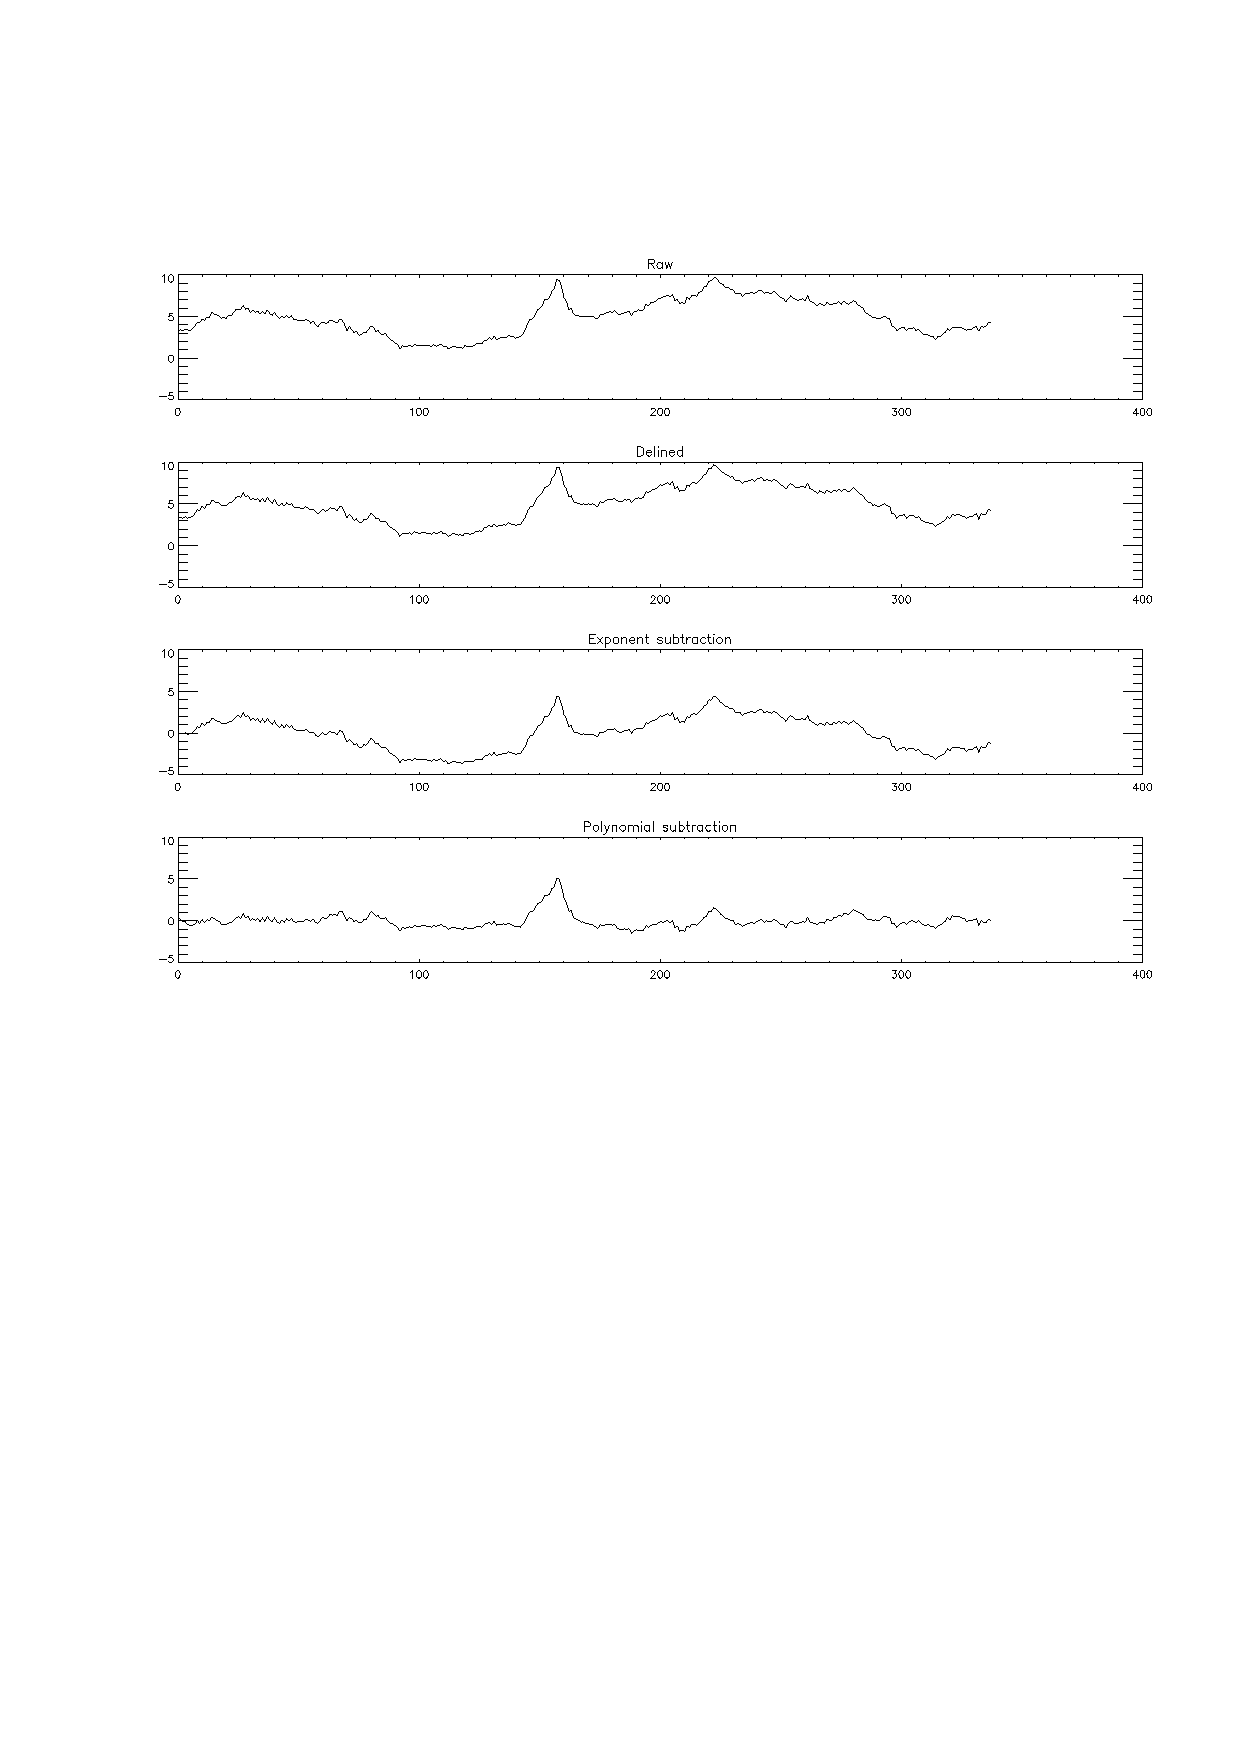
\includegraphics[scale=0.9]{iterative_mapping1}
      \caption{An example of the change in the time series as
      iterative mapping proceeds.  1. Raw time series 2. After removal
      of residual 60Hz signal 3. Exponential decay function at scan
      turnarounds subtracted 4. A polynomial (with astrophysical source
      rejection) is fit to remove large-scale variations across the scan. }
    \end{center}
    \label{fig:IterativeMapping}
  \end{minipage}
\end{figure}

\addtocounter{figure}{0}
\addtocounter{subfig}{1}

  
\begin{figure}
  \begin{minipage}{6.5in}
    \begin{center}
      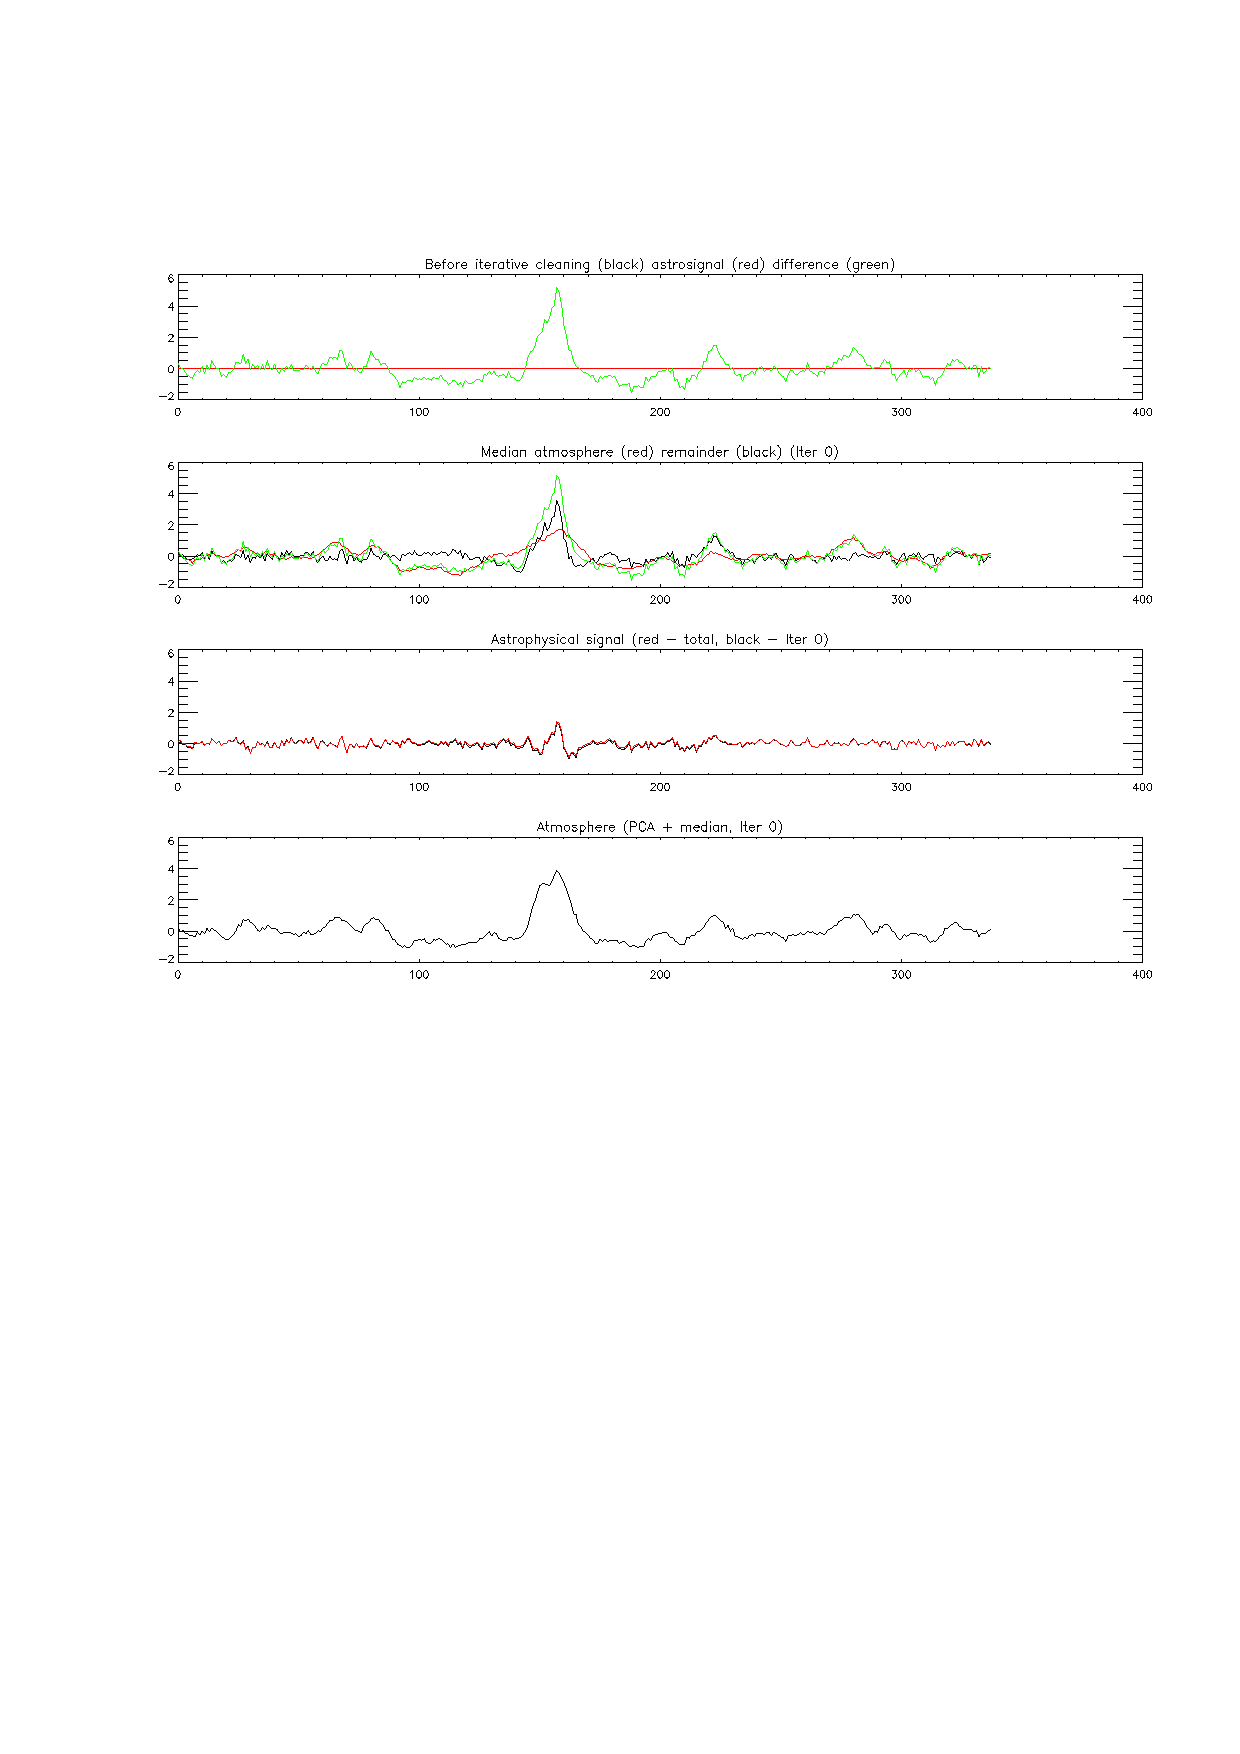
\includegraphics[scale=0.9]{iterative_mapping2}
      \caption{Panel 1 is the same as panel 4 in the previous figure.
      Before the first cleaning, the raw data (black) and remainder data (green)
      are equal because there is no model.  
      Panel 2 shows the median-atmosphere subtraction, which is the first-
      order correction.
      Panel 3 shows the astrophysical signal left over from the PCA selection.
      Panel 4 shows the total atmosphere model from PCA and median estimation}
    \end{center}
    \label{fig:IterativeMapping-b}
  \end{minipage}
\end{figure}

\addtocounter{figure}{0}
\addtocounter{subfig}{1}

\begin{figure}
  \begin{minipage}{6.5in}
    \begin{center}
      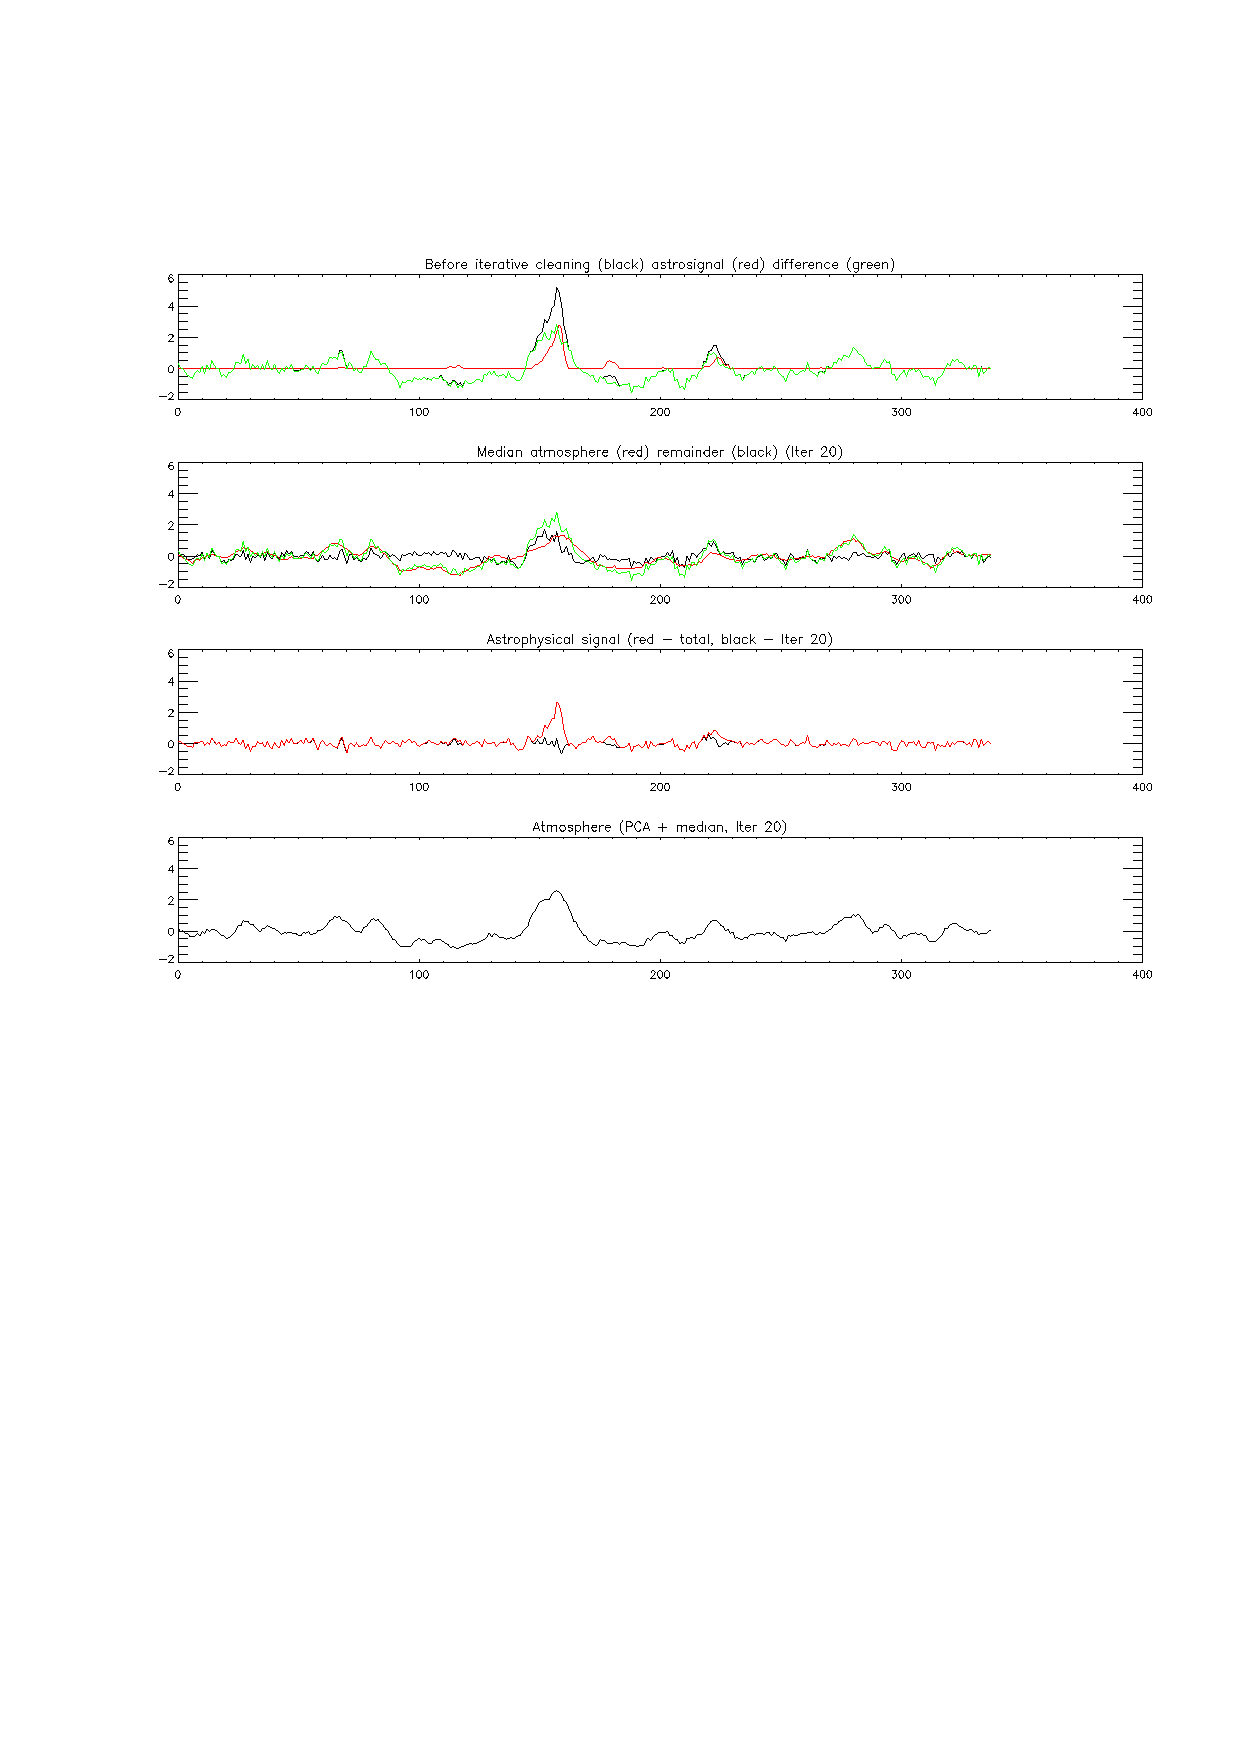
\includegraphics[scale=0.9]{iterative_mapping3}
      \caption{Same as previous figure, except after 20 iterations.
      Panel 1 - The deconvolved astrophysical map is returned to a timestream (red)
      and subtracted from the 'raw' data (black). 
      Panel 2 - The median of the remainder (green) is subtracted as the first
      atmosphere estimation
      Panel 3 - The cumulative astrophysical model (red) and the additional astrophysical
      signal from iteration 20 (black)
      Panel 4 - The atmosphere signal after 20 iterations}
    \end{center}
    \label{fig:IterativeMapping-c}
  \end{minipage}
\end{figure}

% -----------------------------------------------------------------------------
\setcounter{subfig}{1}
\begin{figure}
  \begin{minipage}{3.25in}
    \begin{center}
      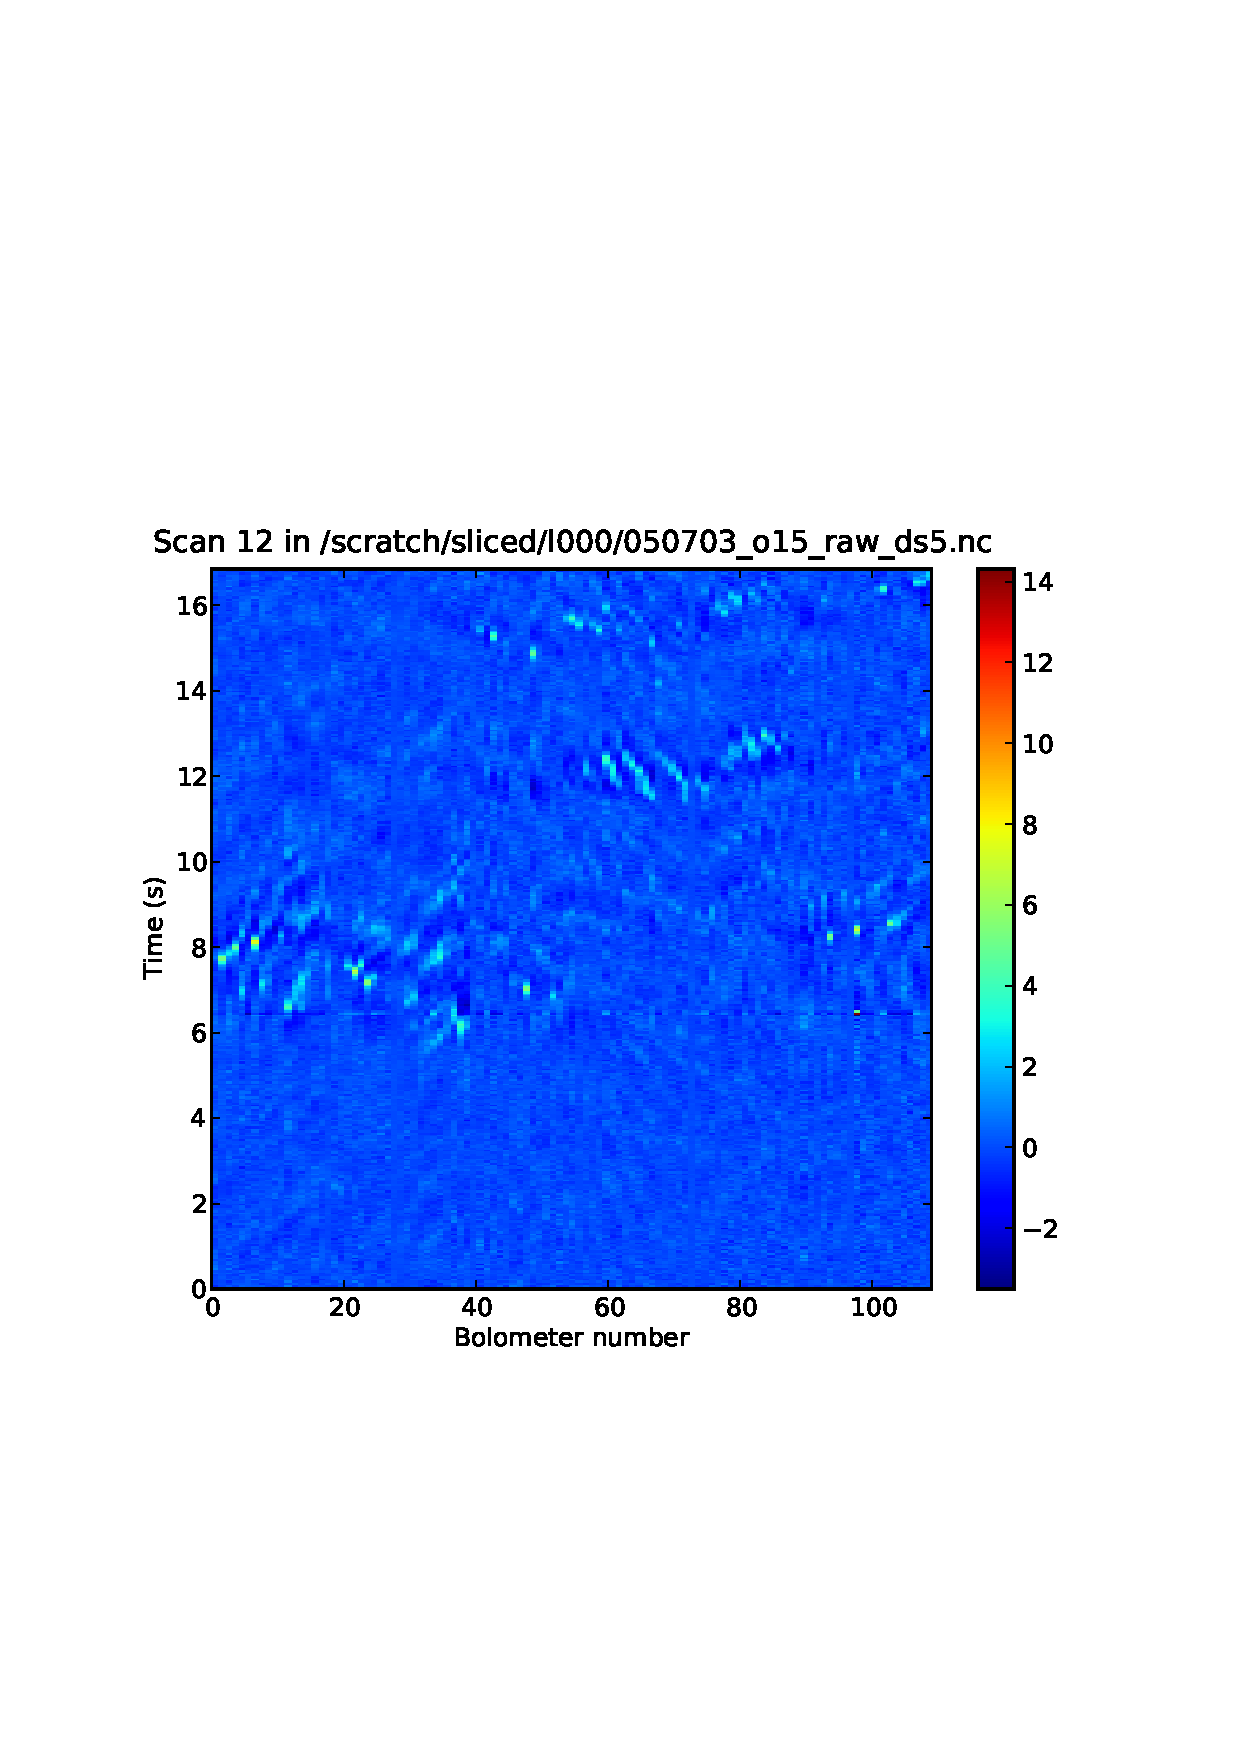
\includegraphics[scale=0.5]{flagger_withglitch}
    \end{center}
  \end{minipage}
  \begin{minipage}{3.25in}
    \begin{center}
      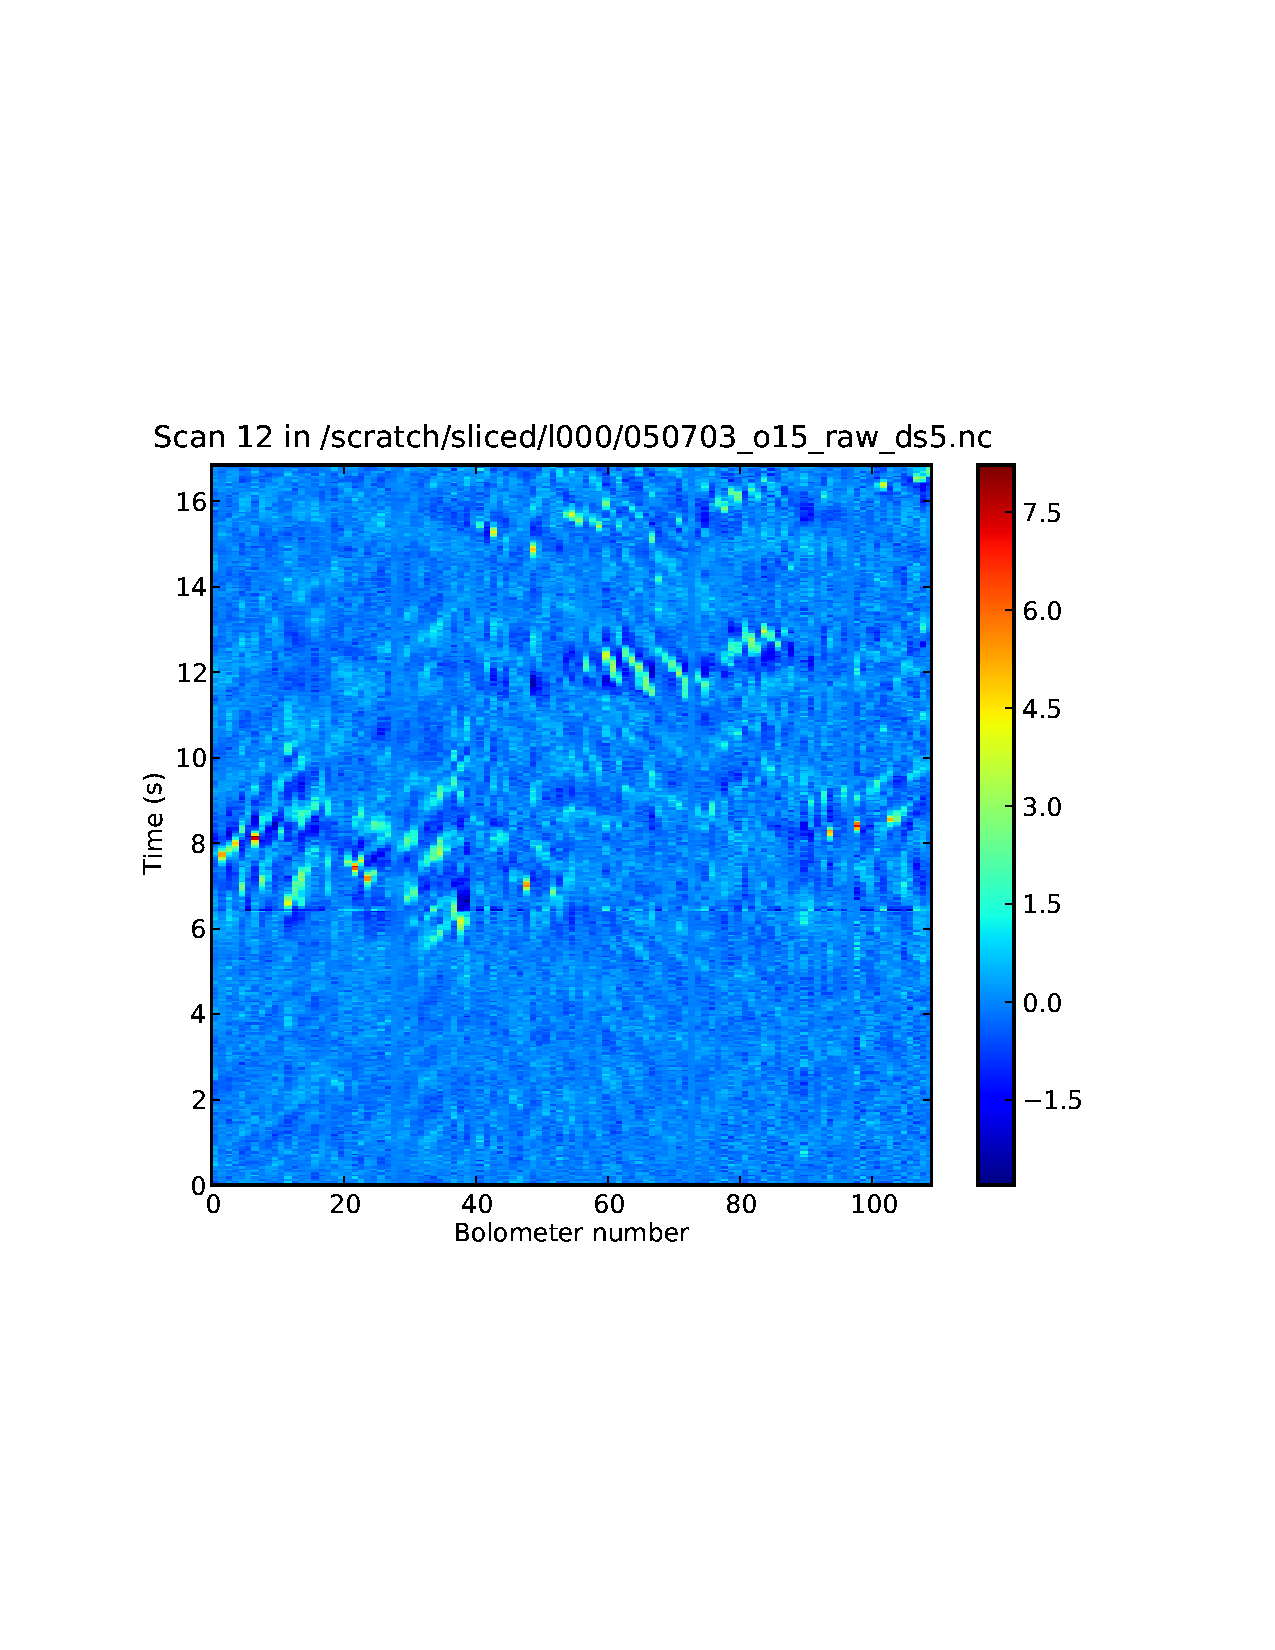
\includegraphics[scale=0.5]{flagger_glitchgone}
    \end{center}
  \end{minipage}
  \caption{An illustration of the flagging process using the waterfall plot.
  Left: The glitch apparent at middle right (bolometer 98, around 6.2s) is the
  same one whose time series is shown in (\em{b}).  Because of
  the PCA subtraction, the effect of the glitch also propagates over the other
  bolometers, appearing as a horizontal stripe. Right: The same data displayed
  with the time point including the glitch flagged out and rescaled}

  \label{fig:Flagger}

  \addtocounter{figure}{0} 
  \addtocounter{subfig}{1}
  
  \begin{minipage}{6.5in}
    \begin{center}
      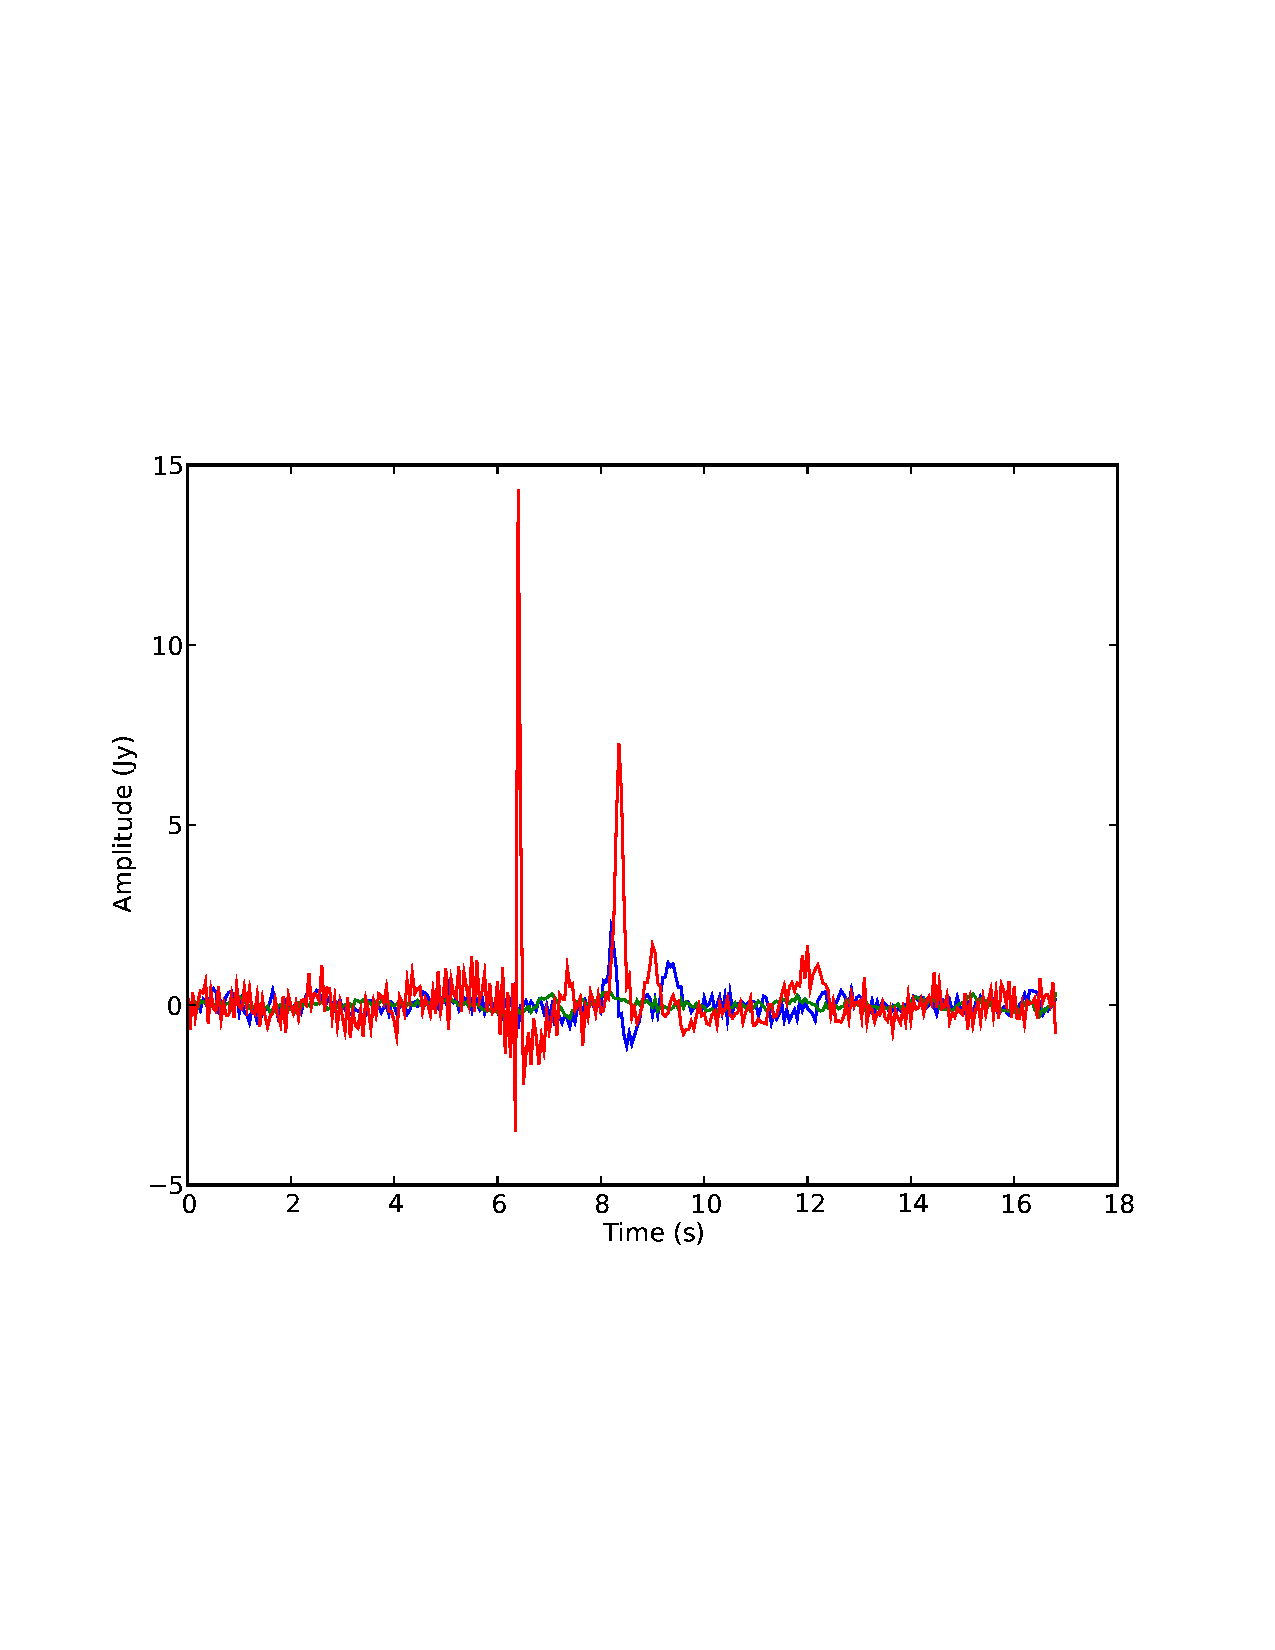
\includegraphics[scale=0.5]{flagger_plots}
      \caption{An illustration of a ``glitch'' in a single bolometer timestream
      (red) due to a cosmic ray strike.  Note the acausal ringing due to the
      application of the downsampling filter.  The time series for a physically
      adjacent bolometer is shown in blue, and a bolometer which does not pass
      over the source in green.  The PCA atmosphere estimation has already been
      subtracted from the data.}
    \end{center}
  \end{minipage}

\end{figure}

% -----------------------------------------------------------------------------

\renewcommand{\thefigure}{\arabic{figure}}

\Figure{crs}{The distribution of glitch amplitudes flagged and removed from the
data in the \lon=111 field.  Glitches below the detection threshold may
contribute to the overall noise.  Each data point represents .1s of integration
time.}{fig:GlitchDistribution}{1.0}

\begin{figure}
  \begin{minipage}{6.5in}
    \begin{center}
      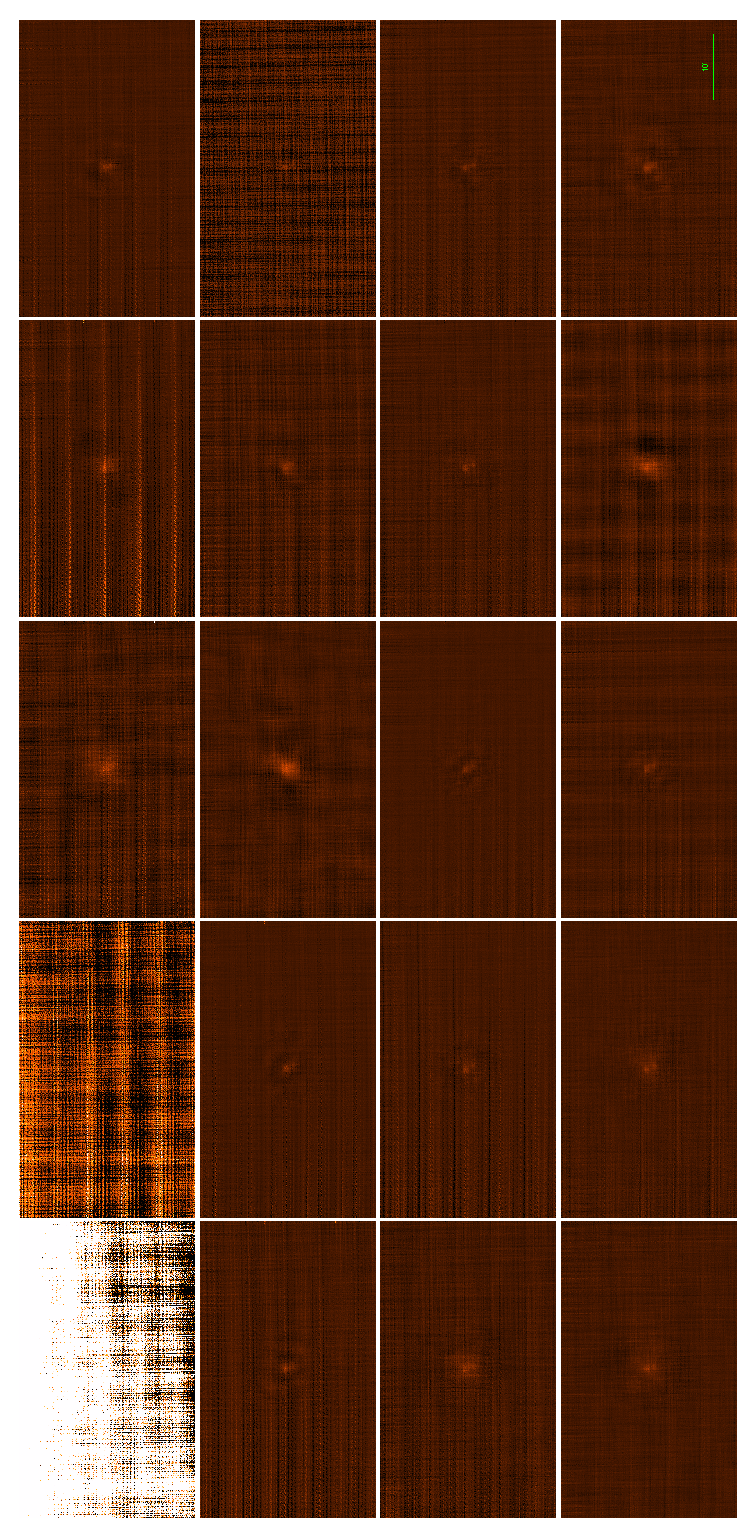
\includegraphics[angle=270,scale=0.6]{eachpca}
    \end{center}
  \end{minipage}
\vspace{0.25in}
  \begin{minipage}{6.5in}
    \begin{center}
      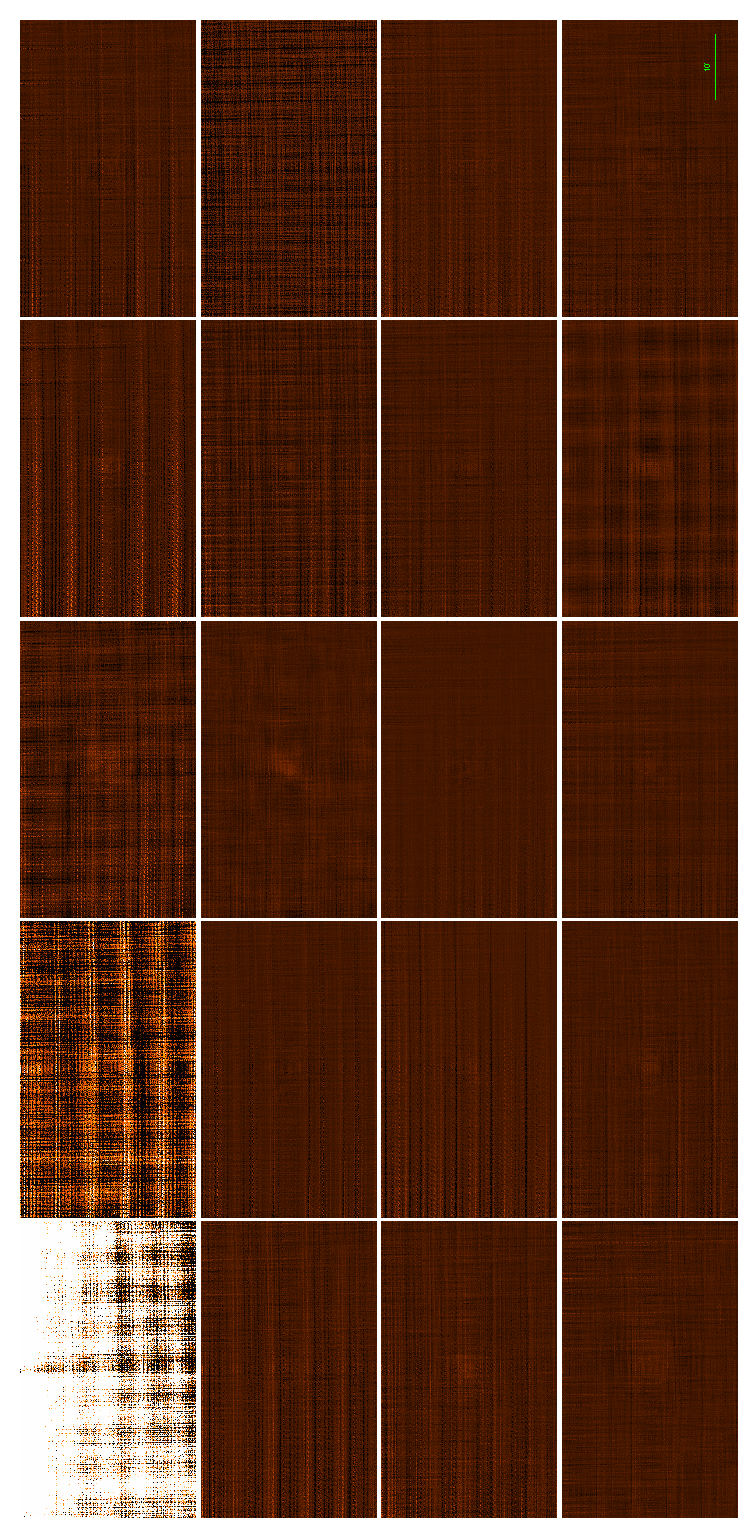
\includegraphics[angle=270,scale=0.6]{eachpca_20iters}
    \end{center}
  \end{minipage}
  \caption{Selected images to illustrate the PCA process.  The
  displays are in Galactic coordinates with a color range from -.1 to
  1.0 \jyb.  {\it Top 4 rows}: a grid of maps of each of the first 20
  PCA components displayed at the same scale.  It is clear that NCG
  7538, the object imaged, has emission in each component.  There are
  varying levels of noise in each component, with the first and second
  being the most obvious atmospheric components.  Most of the other
  noise components are probably detector noise correlated among a
  subset of the bolometers.  The streaks are residuals of the
  scan-turnaround noise that was not removed by the exponential model
  fit.  {\it Bottom 4 rows}: The same figure, but after 20 iterations.
  The figure is the breakdown of the atmosphere remainder (i.e.  the
  raw data minus the astrophysical model) into eigenfunctions.  Very
  little astrophysical flux remains at any level of correlation,
  though there is some at large (few arcminute) scales.}
\label{fig:PCA_Graphical}

\end{figure}

\Figure{l001_deconvolutionkernelcompare}{The effect of deconvolution
on the iterative process can be seen in its effect on the residuals in
these images of Sgr B2, all displayed at the same scale. From left to
right: map, residual, model. Top to bottom kernel size: 14.4\arcsec,
21.6\arcsec, 31.2\arcsec, 7.2\arcsec. The final version of the
pipeline uses 14.4\arcsec, which has the result of leaving no flux in
the residual at the location of Sgr B2, and does not ``dig a hole'' in
the residual map, as the 7.2\arcsec\ kernel does.  The 7.2\arcsec\
kernel also lacks the noise-rejection features of the larger kernels,
as can be seen in the last panel.}{fig:Deconvolution}{1.0}

\Figure{survey_depth}{The depth of the BGPS in the first quadrant as a
function of Galactic longitude.  The black histogram plots the
standard deviation as a function of longitude binned in $0.9\arcdeg
\times 0.9\arcdeg$ degree blocks (to avoid high-noise regions at scan
edges) centered on $b=0$ for the error maps $E$.  Red is similar, but
the estimator is median(1/sqrt(weight
map).}{fig:NoiseVsLongitude}{1.0}

% -----------------------------------------------------------------------------

\clearpage

\FigureTwo{pca_comparison_nolegend_l111}{deconvolution_comparison_nolegend_l111}{The
fractional flux recovered as a function of source size for
well-separated Gaussian sources with FWHM as indicated.  \emph{Left}:
3 (blue), 7 (green), 10 (yellow), 13 (orange), 16 (red), 21 (teal), 26
(lime), 31 (black) PCA components subtracted.  Note that flux recovery
drops to 50\% at 120\arcsec for the 13 PCA component cleaning used in
the released data.  The 3 and 7 PCA cases show bumps because
atmospheric noise is still present at large scales.  The $>$100\%
recovery for simulated sources smaller than the deconvolution kernel
is a side-effect; since the deconvolution kernel is smaller than the
beam, no real astrophysical source should ever be smaller than the
kernel.  \emph{Right}: 7.2\arcsec (cyan), 14.4\arcsec (black),
21.6\arcsec (red), 31.2\arcsec (green) deconvolution kernel for 13 PCA
components subtracted.  It is clear that the larger deconvolution
kernels generate spurious signal at smaller scales, but the flux
recovery is very close to 1 at the beam size
(\bcamfwhm)}{fig:PCA_Filter}{1.0}

\Figure{image_types}{Examples of four of the image types being
released.  Axes are offsets in arcminutes.  See section
\ref{sec:FinalMaps}. Top left: Map.  Top right: Residual.  Bottom
left: Deconvolved.  Bottom right: Weight}{fig:sampleimages}{1.0}

\clearpage

% -----------------------------------------------------------------------------
%\begin{sidewaysfigure}[h]
\begin{figure}
% This assigns the correct label to the *entire* Figure 2.
  \caption{Images from the BGPS.}
  \label{fig:BGPSMontage}
  \addtocounter{figure}{-1}
  \renewcommand{\thefigure}{\arabic{figure}\alph{subfig}}  
  \begin{minipage}{6.5in}
    \begin{center}
      \includegraphics[scale=0.9]{fig1_pg1_bw_inv_bar_label}
      \caption{$\lon=-10.5$ to $\lon=19.5$ Units are \jyb.  The
      brightest sources, e.g. Sgr B2, Sgr A, and sources near
      $\lon=10$ and $\lon=13$, appear to be saturated, but this is
      only a display artifact.  The noise is more pronounced from
      $\lon=-7$ to $\lon=-2$ because this region was observed less.}
    \end{center}
  \end{minipage}
\end{figure}

\addtocounter{figure}{-1}
\addtocounter{subfig}{1}

\begin{figure}
  \begin{minipage}{6.5in} 
    \begin{center}
      \includegraphics[scale=0.9]{fig1_pg2_bw_inv_bar_label} 
      \caption{$\lon=19.5$ to $\lon=49.5$.  Units are \jyb .
	G34.3+0.15, W 51, W 43, W 49, and M 17 appear to be saturated,
	but this is only a display artifact.  The $20 < \ell < 40$
	region through the 4-8 kpc molecular ring and approximately
	the termination of the galactic bar is particularly rich in
	clumps.}
    \end{center}
  \end{minipage}
\end{figure}

\addtocounter{figure}{-1}
\addtocounter{subfig}{1}

\begin{figure}
  \begin{minipage}{6.5in} 
    \begin{center}
      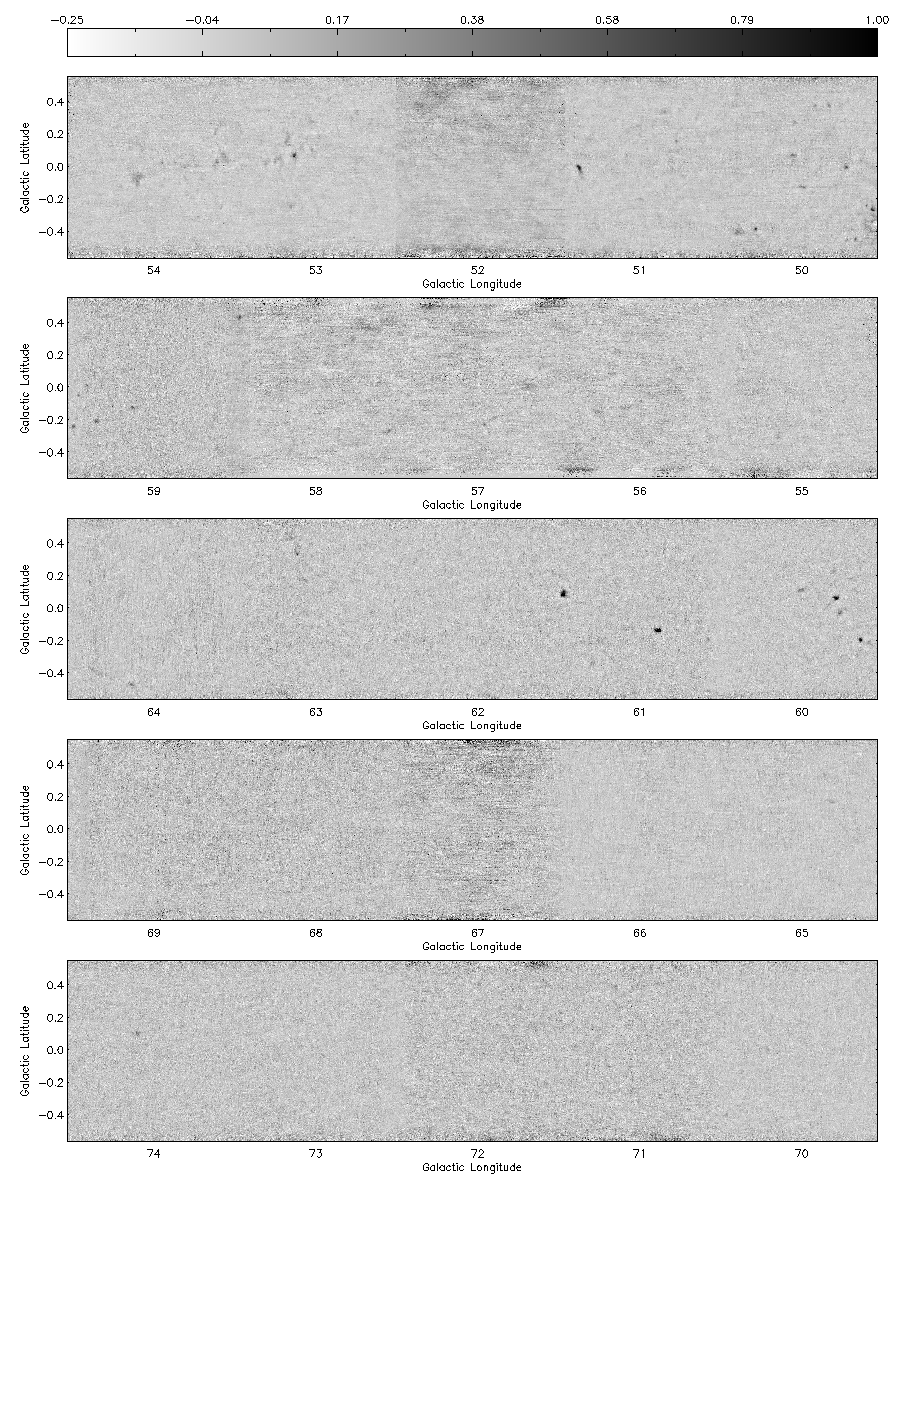
\includegraphics[scale=0.9]{fig1_pg3_bw_inv_bar_label}
      \caption{$\lon=49.5$ to $\lon=74.5$.  In comparison to the inner galaxy, the $65
      < \ell < 75$ has a very sparse population of faint clumps}
    \end{center}
  \end{minipage}
\end{figure}

\addtocounter{figure}{-1}
\addtocounter{subfig}{1}

\begin{figure}
  \hspace{-1in}
  \includegraphics[scale=0.8]{fig1_pg5_bw_inv_bar_label} 
  \caption{The Cygnus Arm. Note that coverage in \emph{b} is extended to $\pm
  1.5\deg$. The large scale `peanut' shape including DR21 is suggestive of a
  large wind-blown bubble, although.... [John: fill in discussion here or we'll
  remove it].  See section \ref{sec:motte} for a comparison with the
  \citet{motte07} IRAM study of this region. }
\end{figure}
%  \vspace{-4in}

\addtocounter{figure}{-1}
\addtocounter{subfig}{1}

\begin{figure}
\hspace{-0.5in}
  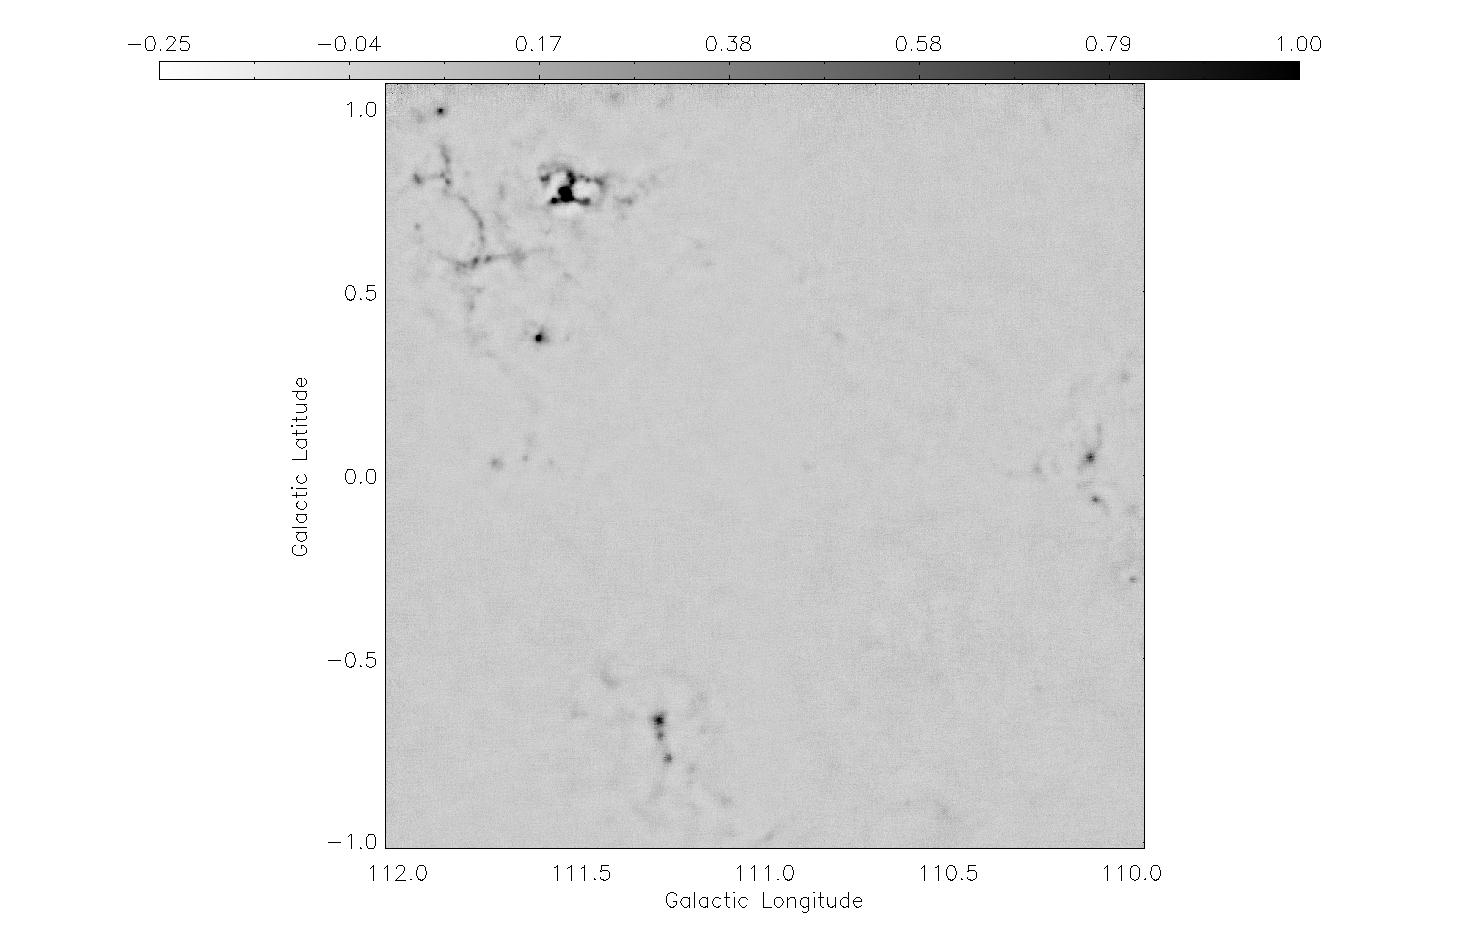
\includegraphics[scale=0.8]{fig1_pg4_bw_inv_bar_label} 
  \caption{Cloud complexes centered at $\lon=111$ in the Perseus Arm. 
  The NGC 7538 complex is in the upper-left.}
\end{figure}

\addtocounter{figure}{-1}
\addtocounter{subfig}{1}

\begin{figure}
  \hspace{-1in}
  \includegraphics[scale=0.8]{fig1_pg6_bw_inv_bar_label} 
  \caption{W3/4/5.  The W3(OH)/W3 Main complex is the bright source
  on the right side of the image.  W5 has one scan performed in RA/Dec
  instead of Galactic coordinates and so has non-uniform noise properties
  in each square degree}
\end{figure}

\renewcommand{\thefigure}{\arabic{figure}}

\clearpage

\Figure{bgps_glimpse_vgps_28_5}
{An RGB image of a portion of the Galactic Plane, combining Bolocam
(red), VGPS 20 cm continuum (green) and Spitzer GLIMPSE 8 \mum\
(blue).}  {fig:Science}{1.0}

\clearpage



